\section{Singapore, Stamps and Postal history}

This is a survey of the postage stamps and postal history of Singapore.
Singapore is an island city-state off the southern tip of the Malay Peninsula, 137km north of the equator, south of the Malaysian state of Johor and north of Indonesia's Riau Islands. Singapore is the smallest nation in Southeast Asia.

The island rose in importance during the 14th century and became an important port until it was destroyed by Portuguese raiders in 1613. In 1819 the Englishman Sir Thomas Stamford Raffles established a British trading post on the island. Under British colonial rule, Singapore grew in importance rapidly becoming a major port city. During World War II, Singapore was occupied by Japan from 1942 to 1945. After the war, Singapore reverted to British control, with increasing levels of self-government being granted, culminating in Singapore's merger with the Federation of Malaya to form Malaysia in 1963. Singapore became an independent republic on 9 August 1965.


\subsection{Straits Settlements}

Main article: Postage stamps and postal history of the Straits Settlements
Singapore was originally part of the Straits Settlements and used their stamps until 1942.


\subsection{Japanese occupation}

During World War II, Singapore was occupied by the Japanese between 1942 and 1945.


\subsection{British Military Administration}

After the surrender of the Japanese Occupation forces at the end of World War II, Singapore and Malaya were administrated by the British Military Administration (BMA). Free postage was implemented for a short period from 17 Sept 1945 till 18 Oct 1945. On 19 Oct 1945, Straits Settlements stamps overprinted B.M.A. MALAYA were issued for postal use. These stamps were used till 1948, when the first Singapore stamps were issued.


\subsection{Crown colony}

Singapore became a British Crown Colony from 1946 until 1959.[1] The first stamps of Singapore were issued on 1 September 1948[1] and were similar to stamps of the Straits Settlements, but inscribed SINGAPORE at the foot.[2] Stamps were issued for the omnibus series of the Royal Silver Wedding (1948), 75th Anniversary of the Universal Postal Union (1949) and the Coronation of Queen Elizabeth II (1953).[2]


\subsection{State of Singapore}

From 3 June 1959, Singapore became a self-governing state as the State of Singapore. Five sets of commemorative stamps were issued in this period, to mark the New Constitution in 1959 and National Days in 1960, 1961, 1962 and 1963. All were inscribed State of Singapore. In addition a long definitive set marked simply Singapore was issued from 1962 onwards.[2]

\subsection{Federation of Malaysia}

In 16 September 1963 Singapore merged with the Federation of Malaya along with Sabah and Sarawak to form the Federation of Malaysia.[1]

\subsection{Independence}

On 9 August 1965, Singapore seceded from the Federation of Malaysia to become an independent republic within the British Commonwealth.[1] 

A set of stamps were issued in 1966 to commemorate the first anniversary of independence marked Republic of Singapore but all later stamps to this day have been marked just Singapore.[2]

\begin{figure}[htbp]
\centering
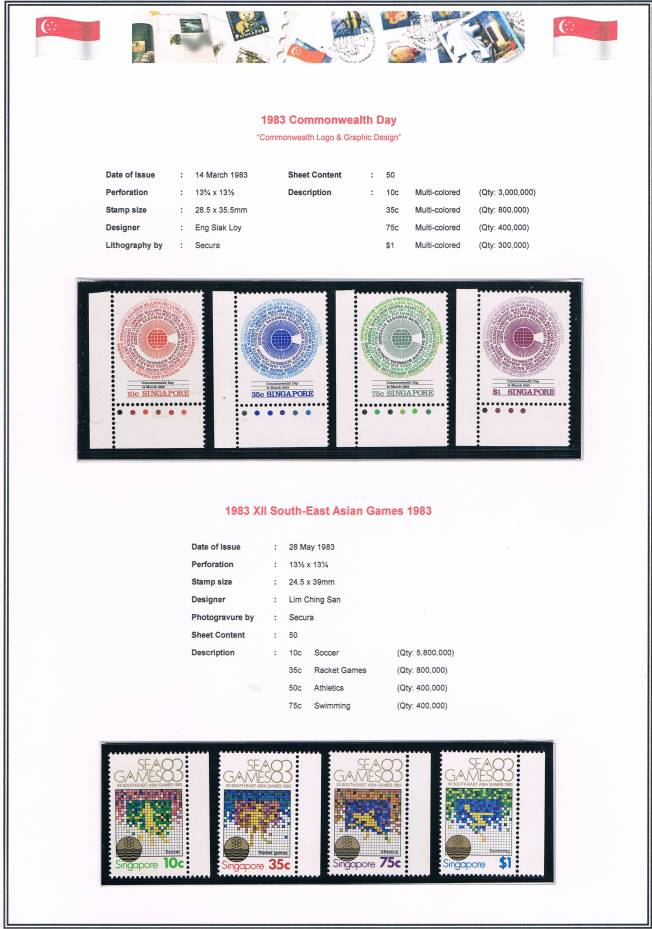
\includegraphics[width=.90\textwidth]{../singapore/1983-01.jpg}
\caption{1983 issues }
\end{figure}

http://singpost.wordpress.com/2012/10/03/singapore-stamp-year-1983/                